\section{Resultados}
\subsection{Discos de Magdeburg}

%TODO: formatar e, talvez mudar algumas coisas de seção

%TODO: Algumas coisas estõa fora de lugar, aqui falamos de resultados. 
% Qual a razão para ter uma discussão aqui? -TF8

Durante o experimento, os hemisférios foram encaixados e alinhados (\cref{foto hemisferios}). % metodologia?
Posteriormente, ao serem puxados em direções opostas (por forças de tração) eles não se separaram nem apresentaram deformação notável, indicando que tais forças não superaram aquelas que os uniam. % Na minha humilde opinião, daqui pra cima é resultado, daqui pra baixo é discussão
Tal resultado pode ser explicado pelo fato de que entre discos ocorre um vácuo (sem possibilidade de entrada de ar), logo por fora há a pressão atmosférica pressionando-os, sendo que ela não é contrabalanceada por uma pressão interna, sendo essa segunda mínima.

\begin{figure}[H]
    \centering
    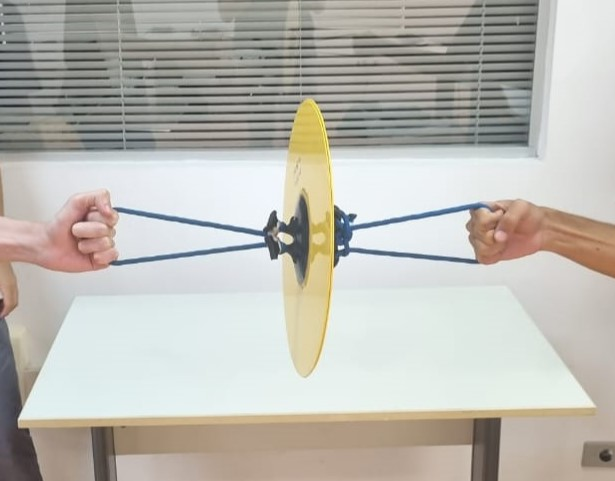
\includegraphics[width=0.5\textwidth]{fig/Cortada.jpeg}
    \caption{Hemisférios sob tração}
    \label{foto hemisferios} % TF8: Péssima label
\end{figure}
Foi feito também um diagrama (\cref{esquema hemisférios}) das forças que atuam sobre um dos hemisférios no eixo horizontal (em que é feita a tração).

\begin{figure}[H]
    \centering
    \includegraphics[width=0.5\textwidth]{fig/Diagrama de forças hemisferio.png}
    \caption{Esquema dos hemisférios sob tração. Em que Fa é a força feita pela pressão atmosférica; Fh2 é a força aplicada pelo segundo hemisfério sobre o analisado, por ser pressionado pela pressão atmosférica; T é tração feita pelos estudantes que puxavam os hemisférios.}
    \label{esquema hemisférios}
\end{figure}

%TODO: Melhorar essa legenda -TF8

Como o sistema encontrava-se em equilíbrio estático, pode-se concluir que, em módulo, \(Fa = Fh2 + T\). Além disso, dado que a pressão atmosférica é constante e a área dos discos também (logo \(Fa\) é fixa), pode-se concluir que \(Fh2\) deve reduzir proporcionalmente ao aumento da tensão \(T\). Por fim, para separar os discos, seria necessária uma tração, em cada lado (se iguais) superior à força atmosférica:

\begin{align*}
    Fa = \text{pressão} \cdot\text{área}\\
    \text{Área} = 9,62 m^2 \cdot 10^{-2}\\
    \text{Pressão atmosférica*} = 9,235 \cdot 10^4 Pa = N/m^2\\
    Fa = (9,235 \cdot10^4) \cdot 9,62 \cdot 10^{-2} = 8,88407 \cdot 10^3 N  
\end{align*}

	Logo, a força de cada lado para separar os discos seria de \(8,884 \cdot 10^3 N\). Isto é, aproximadamente equivalente a pendurar \(9,06 \cdot10^3\) kg na esfera.
 
	%TODO: transformar isso em uma footnote?
    % TF8: De acordo.
    *Foi utilizada a pressão atmosférica medida pelo Instituto de Astronomia, Geofísica e Ciências Atmosféricas da Universidade de São Paulo %TODO: citar a ref de baixo aqui 

    %TODO: Por isso aqui como referência(de 923.5 hPa em 30/3/2025, http://www.estacao.iag.usp.br/index.php).
    % TF8: De acordo.
    
	Cálculo de erro: a área foi calculada a partir do diâmetro do hemisfério, de 35cm, cujo erro associado é \(\sigma_R = \pm0,5cm = \pm0,5\times10^{-2}m\). Enquanto o erro associado à pressão atmosférica é \(\sigma_P = \pm 5\) Pa.

    %TODO: Arrumar esse texto -TF8

	Por propagação de incerteza (tome R como raio e P como pressão):

\begin{align*}
&\sqrt{\left( \frac{\partial }{\partial R} R^{2}\pi P \times\sigma_R \right)^{2} + \left( \frac{\partial }{\partial P} R^{2}\pi P \cdot\sigma_P \right)^{2}}\\
&= \sqrt{\left( 2 \cdot 0,175 \pi 92350 \cdot 0,005 \right)^{2} + \left(0,175^{2}\pi \cdot 5 \right)^{2}} \\
&\cong  \pm 5,07 \cdot 10^2 N
\end{align*}

    Dessa forma, podemos afirmar com mais precisão que seriam necessários \(8884,07 N \pm 507 N\) de força para separar as esferas. 

\subsection{Frasco com membrana}

    Após análise com o software Traker, obtemos a \cref{copo.png}. Veja
    \begin{figure}[H]
        \centering
        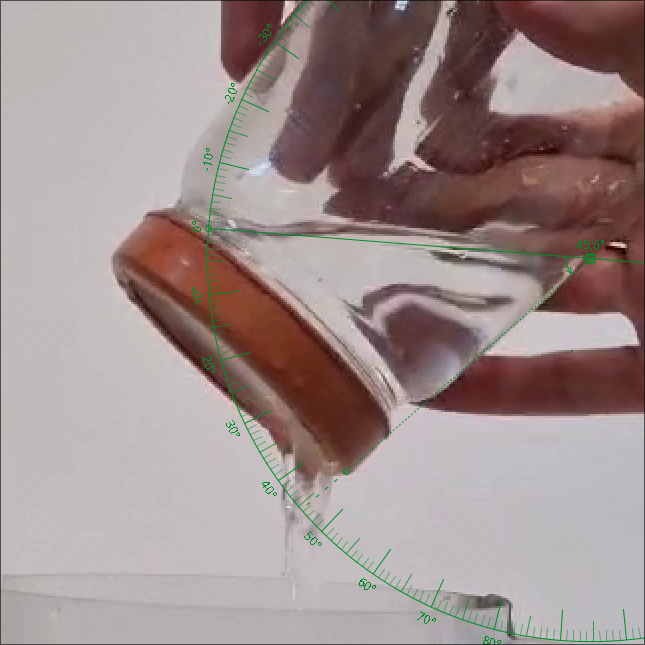
\includegraphics[width=.5\linewidth]{fig/copo.png}
        \caption{Ângulo de inclinação do copo para equilíbrio de pressões}
        \label{copo.png}
    \end{figure}

    Note a inclinação do frasco em relação ao nível da água, em torno de \( 45,6 \)° .

\subsection{Manõmetros}

Para este experimento, vamos avaliar os valores da seguinte maneira:
\begin{enumerate}
    \item Vamos nomear de Extremidade da Atmosfera, E. Atm, a ponta do tubo em U que está exposta ao ar;
    \item Vamos nomear de Extremidade do Recipiente, E. Recip, a ponta do tubo em U na qual se conecta o cano móvel a ser submerso no recipiente;
    \item Vamos nomear de Extremidade Livre, E. Livre, a ponta de vidro de diâmetro maior do cano móvel que submergimos no líquido;
    \item Vamos corrigir os valores medidos na E. Livre para que represente quantos centímetros abaixo da água está a ponta.
\end{enumerate}

% TODO: Isso não é metodologia? -TF8

Dessa forma, os valores obtidos estão sintetizados na \cref{tab_man}

\begin{table}[H]
    \centering
    \begin{tabular}{c | c | c}
        \hline
        \textbf{E. Livre (cm \(\pm 0,5\))} & \textbf{E. Atm (cm\(\pm 0,5\))} & \textbf{E. Recip (cm \(\pm0,5\))}\\
        \hline
        0,0 & 12,2 & 12,2\\
        \hline
        5,0 & 14,5 & 11,1\\
        \hline
        10,0 & 16,2 & 9,0\\
        \hline
    \end{tabular}
    \caption{Valores mensurados com o manômetro de tubo aberto}
    \label{tab_man}
\end{table}

\subsection{Densidade do líquido}
Definindo a linha paralela à separação da fase de água com a fase do líquido misterioso como ponto de altura \(h = 0\), podemos determinar a altura em que a água fica exposta ao ar como \(h_w = \qty{0,123}{m}\) e a altura na qual o líquido misterioso fica exposto ao ar como \(h_l = \qty{0,153}{m}\). Com esses dados, a lei de Stevin nos permite calcular a densidade do líquido misterioso:
\begin{align*}
    \rho_l \cdot h_l &= \rho_w \cdot h_w\\
    \rho_l &= \frac{\rho_w \cdot h_w}{h_l}\\
    \rho_l &= \frac{966,5 \cdot 0,123}{0,153} = \qty{767,0}{kg/m^3} 
\end{align*}

%TODO: Bom -TF8
